\chapter{Impact of the largest systematic uncertainties on \BHee}
\label{app:impacts}

The impact of the largest systematic uncertainties on the observed \Hee branching fraction is shown in Figure~\ref{fig:impacts}. The uncertainties with the largest impact are those affecting the electron energy scale, as well as those affecting the \ggH production cross section. Also shown is the pull of each nuisance parameter, defined as the difference between the postfit and prefit uncertainties, divided by the prefit uncertainty. No significant pulls away from zero are observed.

\begin{figure}[htbp!]
\centering
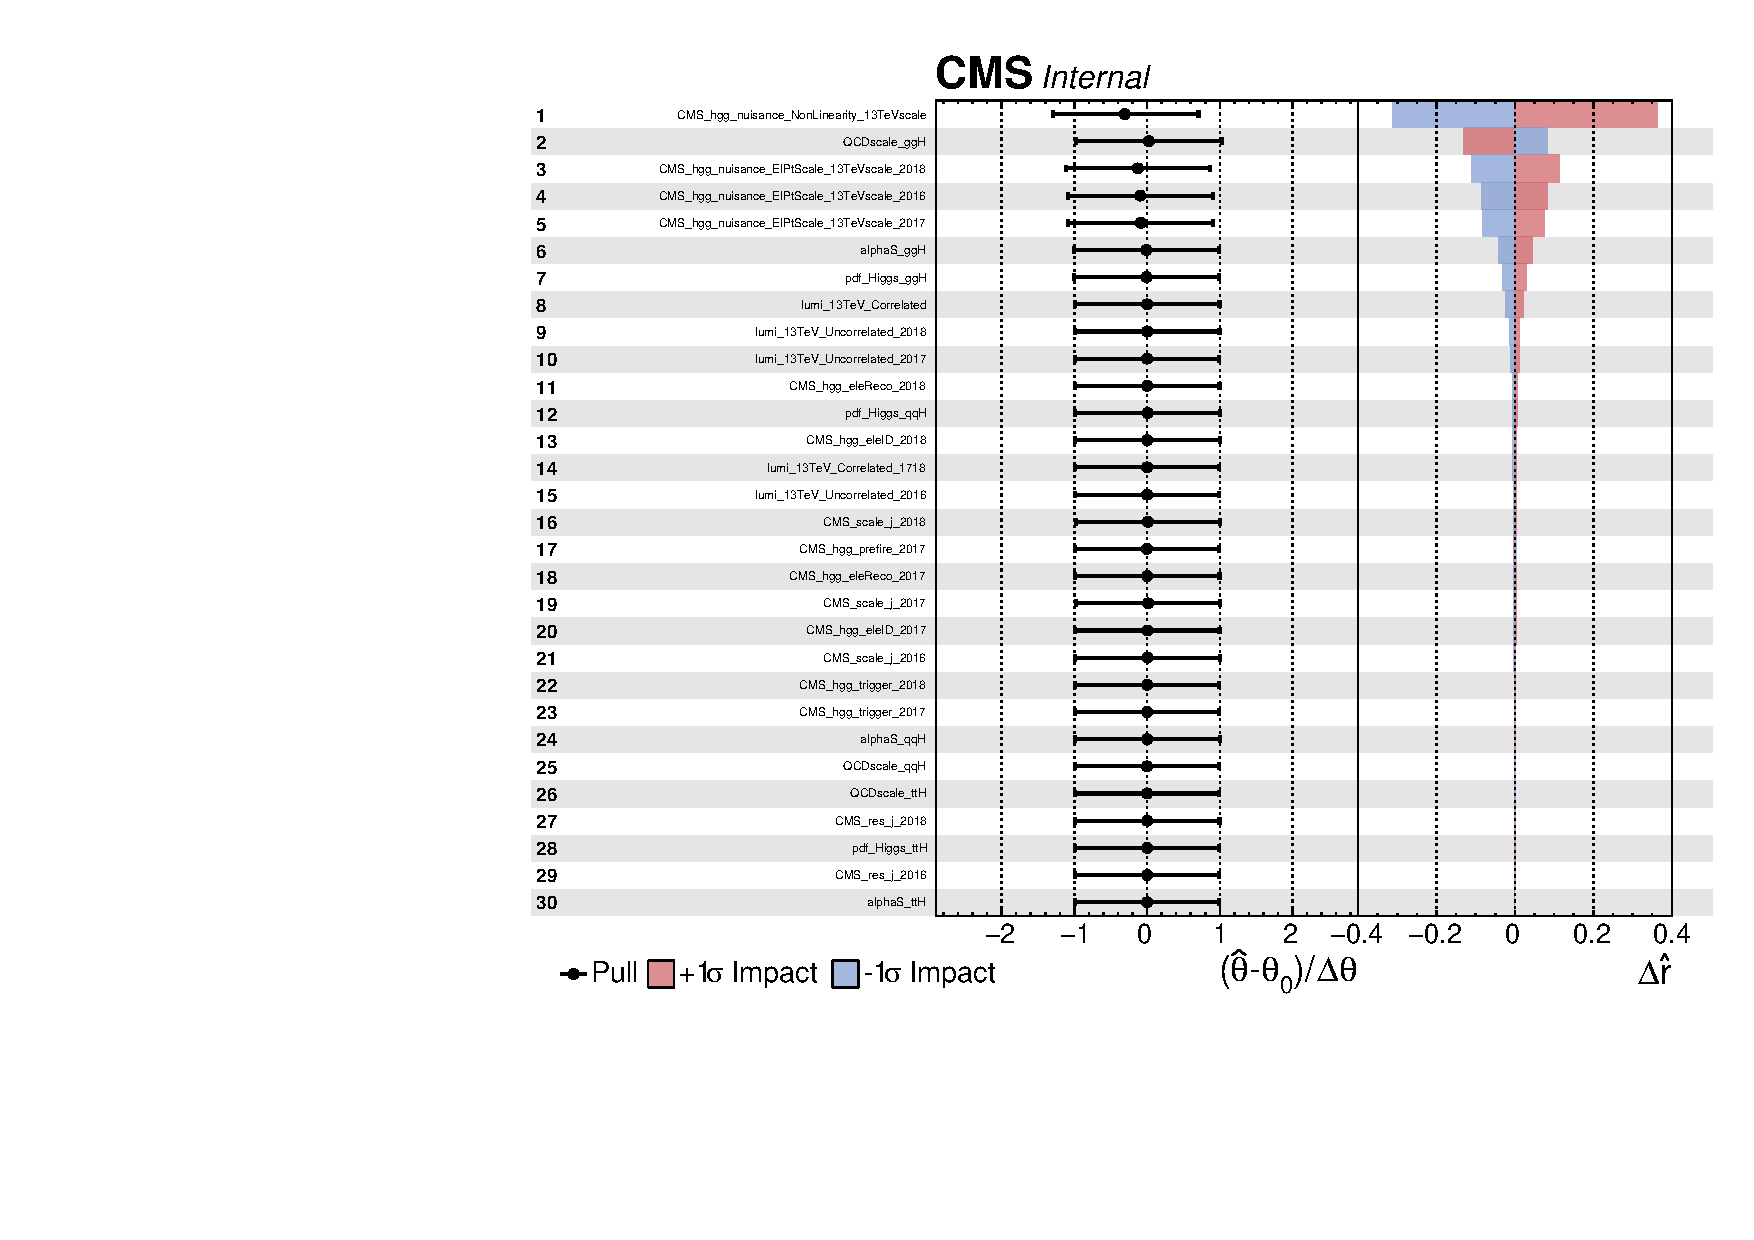
\includegraphics[trim={0cm 0cm 0cm 1cm},clip,width =0.8\linewidth]{Figures/Hee/Results/systs/impacts_pass20_unblinded_dropBkgParams.pdf}\hfill%

\caption[The impact of the top systematic uncertainties on \BHee]{Left: the pull of each nuisance parameter, defined as the difference between the postfit and prefit uncertainties, divided by the prefit uncertainty. The error bar indicates the ratio of the postfit and prefit uncertainties. No significant pulls away from zero are observed. Nuisance paramaters are also not signficantly constrained from the fit. Right: the impact of fixing nuisance parameters to their $\pm1\sigma$ values on the observed \Hee branching fraction (labelled here as $\Delta \hat{r}$).}
\label{fig:impacts}                                              
\end{figure}
